Monte Carlo (MC) methods are a powerful simulation tool that allow scientists to
explore properties of systems that may otherwise by inaccessible via
experimental methods. Monte Carlo methods can be used to solve a variety of
physical problems yielding insight into statistical averages due to random
processes. During the last two decades considerable research has been done on
developing and refining flat-histogram Monte Carlo methods. These Monte Carlo
methods are capable of exploring all of the energy phase space for all
given temperatures in a \emph{single} simulation. In this work, we first
outline the necessary statistical mechanics background. We provide a
description of MC methods and flat-histogram methods, as well as, our newly
developed method SAD (stochastic approximation Monte Carlo with a dynamic
update factor). We discuss physics rich test systems that can be used to
explore the convergence and statistical properties of our newly developed
method SAD.

A driving motivation for developing novel Monte Carlo methods that have
physically based tunable parameters is to provide simulation methods for
exploring porous materials. In this work, we examine the theoretical upper
bound on the storage capacity of porous materials in the context of
light-vehicle fuel storage. We formulate a theoretical upper bound on the
maximum amount of gas that can be stored and released at different pressures.
We propose SAD as a potentially powerful method for examining thermodynamic
properties for porous materials. This body of research serves as a groundwork
for multidimensional SAD which would be able to compute isotherms for any given
porous material thereby providing a powerful way for researchers to determine
the suitability for gas storage applications.

In the following chapters, we follow the manuscript outline with each chapter
corresponding to our published or submitted research on the SAD method applied
to various physical systems, and our work on establishing a theoretical upper
bound on gas storage and delivery for MOFs.

\section{Micro-Canonical Ensemble}\label{micro}
A statistical ensemble is defined as a probability distribution
$\mathcal{P}\left(\Omega\right)$ for the state of the system. The
micro-canonical\index{ensemble!micro-canonical} is a representation for a
system $\Gamma$ that is determined by a fixed number\index{extensive!number
$N$} of particles $N$ (and fixed components $\sum N_i$ for a multi-component
system), a fixed volume\index{extensive!volume $V$} $V$, and a fixed
energy\index{extensive!energy $E$} $E$. All possible states for the system
$\Gamma\left(N,V,E\right)$ have the same number of particles, energy, and
volume due to the system being in isolation from any external environment. The
micro-canonical ensemble\index{ensemble!micro-canonical} is for this reason
also known as the $NVE$ ensemble as the micro-states depend on the
\ind{extensive} macroscopic details.

The probability $\mathcal{P}$ of selecting a micro-state at random for a given range of energies centered about $E$ is given by
\begin{align}
    \mathcal{P} = \frac{1}{\Omega(E)}
\end{align}
where $\Omega(E)$ is the number of micro-states in the system $\Gamma(E)$.

\subsection{The Boltzmann Entropy $S(E)$}\label{entropy}
The Boltzmann entropy $S(E)$ can be defined for any given system $\Gamma$ with discrete energy states by relating it to the microstates:
\begin{align}\label{sdos}
    S(E,V,N) \equiv k_B \ln\Omega(E,V,N)
\end{align}
where the entropy is defined as the logarithm of the density of states and $k_B$ is the Boltzmann constant. An important aspect of this definition in terms of logarithms is that the entropy for multiple isolated systems is additive.
\begin{align}
    S(E_1,E_2) &= k_B \ln(\Omega(E_1)\Omega_2(E_2)) \\
    &= k_B \left( \ln(\Omega_1(E_1)) + \ln(\Omega_2(E_2))\right) \\
    &= \left( S_1(E_1) + S_2(E_2)\right)
\end{align}
From the \nth{1} law of thermodynamics, the system temperature can be written in terms of the density of states by referring to Eq.~\HR{sdos}.
\begin{align}
    \frac{1}{T} = \left(\diff{S(E)}{E}\right)_V = \frac{k_B}{\Omega(E)}\left(\diff{\Omega(E)}{E}\right)_V
\end{align}
The relationship between entropy $S(E)$, $\Omega(E)$, and $T$ will be discussed in further depth in Section~\HR{laws}.

\subsection{Thermodynamics in the Micro-Canonical Ensemble}\label{laws}
The statistical entropy defined in Eq.~\HR{sdos} is consistent with the \nth{1} and \nth{2} laws of
thermodynamics for any system with uniformly distributed microstates.
The \nth{1} law of thermodynamics states that for an isolated system $\Gamma$, the total internal energy is equal to the sum of the heat $Q$ and work $W$ done.
\begin{align}
    \D{U} = \D{Q} + \D{W}
\end{align}
The \nth{1} law follows directly from conservation of energy. The thermodynamic identity states that for any infinitesimal change in the system and fixed number of particles $N$, the internal energy can be written in terms of the entropy.
\begin{align}
    \D{U} =  T\D{S} - p\D{V} \\
    T = \left(\pdv{U}{S}\right)_V
\end{align}

The \nth{2} law of thermodynamics states that for any isolated system $\Gamma$ the entropy $S(E) \geq 0$. The heat of the system can also be related to the entropy using the relation:
\begin{align}
    \delta Q = T\delta S
\end{align}
The relationship between heat and entropy for a system is useful for the \nth{1} law to relate the conjugate variables T, $S(E)$, and $U(E)$.

\section{Canonical Ensemble}
The Canonical ensemble is a representation for a system $\Gamma$ that is
determined by a fixed number of particles $N$ (and fixed components $\sum N_i$
for a multi-component system), a fixed volume $V$, and a fixed temperature $T$.
All possible states for the system $\Gamma\left(N,V,T\right)$ have the same
number of particles, volume, and temperature due to the system being in thermal
equilibrium with a heat bath. The canonical ensemble is for this reason also
known as the $NVT$ ensemble.

The probability $\mathcal{P}$ of selecting a given micro-state $i$ at random is
\begin{align}
    \mathcal{P_i} = \frac{e^{\nicefrac{\left(-E_i\right)}{k_BT}}}{Z}
\end{align}
where $Z$ is the canonical partition function and will be discussed in detail in Section~\HR{betaZ}.

\subsection{The Canonical Partition Function}\label{betaZ}
In statistical thermodynamics $\beta$ is defined as the coldness or the reciprocal of the canonical temperature.
\begin{align}
    \beta = \frac{1}{k_BT}
\end{align}
where $k_B$ is the Boltzmann constant. The partition function for a canonical ensemble can then be written in terms of the Boltzmann factor where $E$ is the total energy of the system in the respective microstate at index $i$.
\begin{align}
    Z = \sum_i e^{-\beta E_i}
\end{align}
The partition function depends both on the microstate energies as well as the
temperature $T$. Because the microstate energies are influenced by microscopic
properties, $Z$ has important statistical meaning.

\section{Thermodynamic Potentials}\label{potentials}
Thermodynamic potentials describe a given thermodynamic state of a given system
and have units of energy $k_BT$. In this section, we will discuss the
thermodynamic potentials ($U$, $F$, $H$, and $G$) and how they are mathematically related through
Maxwell relations. While the internal energy $U(E)$ has been briefly mentioned
in Section~\HR{laws}, we outline in detail the relationship between the state
variables.
\begin{align}
    \D{U(S,V,N)} = T\D{S}-p\D{V}+\mu\D{N}
\end{align}
We can write the temperature $T$, pressure $p$, and chemical potential $\mu$ in terms of derivatives of state variables.
\begin{align}\label{maxU}
    T = \left( \pdv{U}{S}\right )_{V,N}  \quad\quad 
    p = -\left( \pdv{U}{V}\right )_{S,N}  \quad\quad 
    \mu = \left( \pdv{U}{N}\right )_{S,V}  \quad
\end{align}
The Helmholtz free energy $F(T,V,N)$ can be written as follows:
\begin{align}
    \D{F(T,V,N)} = \D{(U-TS)} = -S\D{T}-p\D{V}+\mu\D{N}
\end{align}
We can write the entropy $S$, pressure $p$, and chemical potential $\mu$ in terms of derivatives of state variables.
\begin{align}\label{maxF}
    S = -\left( \pdv{F}{T}\right )_{V,N}  \quad\quad 
    p = \left( \pdv{F}{V}\right )_{T,N}  \quad\quad 
    \mu = \left( \pdv{F}{N}\right )_{T,V}  \quad
\end{align}
The Enthalpy $H(S,p,N)$ can be written as follows:
\begin{align}
    \D{H(S,p,N)} = \D{(U+pV)} = -T\D{S}+V\D{p}+\mu\D{N}
\end{align}
We can write the temperature $T$, volume $V$, and chemical potential $\mu$ in terms of derivatives of state variables.
\begin{align}\label{maxH}
    T = \left( \pdv{H}{S}\right )_{p,N}  \quad\quad 
    V = -\left( \pdv{H}{p}\right )_{S,N}  \quad\quad 
    \mu = \left( \pdv{H}{N}\right )_{S,p}  \quad
\end{align}
The Gibbs free energy $G(T,p,N)$ can be written as follows:
\begin{align}
    \D{G(T,p,N)} = \D{(U+pV-TS)} = -S\D{T}+V\D{p}+\mu\D{N}
\end{align}
We can write the entropy $S$, volume $V$, and chemical potential $\mu$ in terms of derivatives of state variables.
\begin{align}\label{maxG}
    S = \left( \pdv{G}{T}\right )_{p,N}  \quad\quad 
    V = -\left( \pdv{G}{p}\right )_{T,N}  \quad\quad 
    \mu = \left( \pdv{G}{N}\right )_{T,p}  \quad
\end{align}

\subsection{Maxwell Relations}\label{maxwell}
Maxwell's relations are second derivative equalities that relate thermodynamic variables. Maxwell relations are formalism of the Schwarz theorem which states that the order of differentiation is irrelevant.
\begin{align}
    \pdv{}{\theta}\left(\pdv{\Theta}{\phi}\right)=\pdv{}{\phi}\left(\pdv{\Theta}{\theta}\right)
\end{align}
From this theorem and Section~\HR{potentials}, we can derive the most common of Maxwell's relations. The relation involving internal energy $U\left(S,V,N\right)$ relates the natural variables of pressure $p$ and temperature $T$ and can be derived using Equation~\ref{maxU}.
\begin{align}
    \left( {\pdv{U}{S}{V}} \right )_{N} = \left( \pdv{T}{V}\right )_{S,N} = - \left( \pdv{p}{S}\right )_{V,N}
\end{align}
The relation involving the Helmholtz free energy $F\left(T,V,N\right)$ relates the natural variables of entropy $S$ and pressure $p$ and can be derived using Equation~\ref{maxF}.
\begin{align}
    \left( {\pdv{F}{T}{V}} \right )_{N} = \left( \pdv{S}{V}\right )_{T,N} = \left( \pdv{p}{T}\right )_{V,N}
\end{align}
The relation involving the Enthalpy $H\left(S,p,N\right)$ relates the natural variables of temperature $T$ and volume $V$ and can be derived using Equation~\ref{maxH}.
\begin{align}
    \left( {\pdv{H}{S}{p}} \right )_{N} = \left( \pdv{T}{p}\right )_{S,N} =  \left( \pdv{V}{S}\right )_{p,N}
\end{align}
The relation involving the Gibbs free energy $G\left(T,p,N\right)$ relates the natural variables of entropy $S$ and volume $V$ and can be derived using Equation~\ref{maxG}.
\begin{align}
    \left( {\pdv{G}{T}{p}} \right )_{N} = -\left( \pdv{S}{p}\right )_{T,N} = \left( \pdv{V}{T}\right )_{p,N}
\end{align}

\subsection{Thermodynamic Properties}\label{thermoprop}
The Maxwell relations from Section~\HR{maxwell} can be written in terms of thermodynamic properties of the material.  The isochoric heat capacity $C_V$ of a given material is defined as the amount of heat necessary to raise the temperature of the material.
\begin{align}
    C_V = T\left(\pdv{S}{T}\right )_{V,N}
\end{align}
The isobaric heat capacity $C_p$, which is always greater than or equal to $C_V$ according to the Mayer relation, can also be written in terms of the entropy $S$ and temperature $T$ of the system.
\begin{align}
    C_p = T\left(\pdv{S}{T}\right )_{p,N}
\end{align}
The Mayer relation gives the difference of the isobaric and isochoric heat capacities in terms of the thermal expansion coefficient and the isothermal compressibility.
\begin{align}
    C_p - C_V = VT\frac{\alpha^2}{\kappa_T}
\end{align}
The isobaric coefficient of thermal expansion determines to what extent a given material will deform as a result of a change in temperature.
\begin{align}
    \alpha_p = \frac{1}{V}\left( \pdv{V}{T} \right )_{p,N}
\end{align}
Similarly, the isochoric coefficient of thermal expansion can be written as
\begin{align}
    \alpha_V = \frac{1}{p}\left( \pdv{p}{T} \right )_{V,N}.
\end{align}
The compressibility determines to what extent a given material will change volume based on the pressure applied to the system.  The isothermal compressibility can be written:
\begin{align}
    \kappa_T = -\frac{1}{V}\left( \pdv{V}{p} \right )_{T,N}.
\end{align}
Similarly, the isentropic compressibility can be written as
\begin{align}
    \kappa_S = -\frac{1}{V}\left( \pdv{V}{p} \right )_{S,N}.
\end{align}
A major driving force behind introducing the concepts of thermal expansion and compressibility is the ability to write complex derivatives in terms of these parameters. The internal energy derivative and entropy derivative can be written in terms of both the isothermal compressibility and the thermal coefficient of expansion.
\begin{align}
    \left( \pdv{U}{p} \right )_{V,N} = \frac{\kappa_T C_p}{\alpha} - \alpha TV \quad\quad
    \left( \pdv{S}{p} \right )_{V,N} = \frac{\kappa_T C_p}{\alpha T} + \alpha V
\end{align}
Additionally, the enthalpy derivatives can be written in terms of both the isothermal compressibility and the thermal coefficient of expansion.
\begin{align}
    \left( \pdv{H}{T} \right )_{V,N} = C_p + \frac{\alpha V}{\kappa_T}\left(1-\alpha T\right) \quad\quad
    \left( \pdv{H}{p} \right )_{V,N} = \frac{\kappa_T C_p}{\alpha} + V\left(1-\alpha T\right)
\end{align}
Finally, the Gibbs free energy derivatives can be written in terms of the isothermal compressibility, the thermal coefficient of expansion, and the entropy.
\begin{align}
    \left( \pdv{G}{T} \right )_{V,N} = \frac{\alpha V}{\kappa_T}-S \quad\quad
    \left( \pdv{G}{p} \right )_{V,N} = V-\frac{\kappa_T S}{\alpha}
\end{align}

\section{Grand Canonical Ensemble}
The grand canonical ensemble is a representation for a system $\Gamma$ that is determined by a fixed chemical potential $\mu$, a fixed volume $V$, and a fixed temperature $T$. All possible states for the system $\Gamma\left(\mu,V,T\right)$ have the same chemical potential, volume, and temperature due to the system being in thermal and chemical equilibrium with a given reservoir.
The grand canonical ensemble is for this reason also known as the $\mu VT$ ensemble.

The probability $\mathcal{P}$ of selecting a given micro-state at random is
\begin{align}
    \mathcal{P} = e^{\nicefrac{\left(\Phi + \mu N-E\right)}{k_BT}}
\end{align}
where $\Phi\left(\mu,V,T\right)$ is the grand potential of the system $\Gamma$. The grand potential is often referred to as the Landau potential and written:
\begin{align}
    \Phi \equiv F -\mu N = U - TS -\mu N
\end{align}

\subsection{Chemical Potential $\mu$}
The chemical potential $\mu$ of a given system $\Gamma$ is representative of the energy that can be gained or lost due (often because of a phase transition) to a change in the conjugate variable particle number $N$. Analogous to potential energy, higher chemical potential drives particles to lower potential (thereby usually changing the particle number). The chemical potential $\mu_i$ of species $i$ can be represented using a variety of free energies (all of which are equivalent).
\begin{align}
    \mu_i = \left( \pdv{G}{N_i}\right )_{T,P,N_{j \neq i}}  \quad
    \mu_i = \left( \pdv{H}{N_i}\right )_{S,P,N_{j \neq i}}  \quad
    \mu_i = \left( \pdv{F}{N_i}\right )_{T,V,N_{j \neq i}}  
\end{align}

\subsection{Grand Potential and Thermodynamic Quantities}
A variety of important thermodynamic quantities can be written in terms of the grand potential. In differential form, the grand potential can be written as the following (for a single component system $\Gamma$):
\begin{align}
    \D{\Phi(\mu,V,T)} = -S\D{T}-p\D{V}-N\D{\mu}
\end{align}
The number $N$, pressure $p$, and Gibbs entropy $S$ can be written in terms of the grand potential.
\begin{align}
    N = -\left( \pdv{\Phi}{\mu}\right )_{T,V}  \quad
    p = -\left( \pdv{\Phi}{V}\right )_{T,\mu}  \quad
    S = -\left( \pdv{\Phi}{T}\right )_{V, \mu} 
\end{align}


\section{Monte Carlo Simulation}\label{monte}
Experiment and simulation are both necessary to help form a more complete
understanding of our knowledge of how the universe works. Computational
`experiments' such as Monte Carlo methods aid in this understanding by allowing
scientists to explore system configurations that are not easily accessible to
traditional experiment.

In the field of statistical physics, Monte Carlo methods are used to determine
equilibrium properties (thermal averages) of multi-particle systems. A number
of Monte Carlo simulations have been developed over the last century. Some of
these methods are completely unique while others are more sophisticated
variants of an original method. All of the methods share a number of
similarities including picking random moves (we will discuss this process in
Section~\HR{rng}) and determining the acceptance or rejection of a move based
on a probability distribution. They differ primarily in how they explore phase
space and thus compute thermodynamic properties such as the density of states
$\Omega(E)$. The accuracy of any MC simulation depends on the details of how
the system is `explored'. To reduce the error in simulation one can in
principle simply continue to allow the simulation more time to explore phase
space.

The motivation for new research into developing MC methods stems from the
desire to solve ever-increasingly complex physical problems in a faster
simulation time. Many of the originally developed MC methods are unable to
effectively explore the complex phase space of real (and even many test)
systems. Flat-histogram methods (introduced in Section~\HR{fhm}) are able to
explore all energies and temperatures in a `single' simulation. In addition,
they are able to explore complex energy landscapes without getting `stuck'
(either never converging or converging at such a slow rate as to not
practically converge). Many of these flat-histogram methods also have proven
convergence on the statistical error thus guaranteeing convergence. In the
following sections, we will discuss a number of MC methods including importance
sampling and flat-histogram methods introduced in Section~\HR{cmc} and
~\HR{fhm}.

\subsection{Random Number Generation}\label{rng}

Since Monte Carlo moves are inherently stochastic in nature, it is imperative
that any useful random number generator be fast and ideally non-deterministic.
In practice, pseudo-random number generators (PRNGs) are used in order to
generate the fast random streams although they are deterministic. In order for
a PRNG to be acceptable for use in Monte Carlo simulation it must meet certain
criteria~\cite{sawilowsky2003you}. First, the PRNG must have a long `period'
before repeating values. Poor PRNGs (that is ones with short periods) can lead
to systematic error in Monte Carlo simulations~\cite{ferrenberg1992monte,
plascak2002cluster, ossola2004systematic}. Second, the PRNG must actually be
able to pass certain statistical tests such as implemented in the TestU01
library~\cite{l2007testu01}.

There are a variety of PRNGs each with benefits and few without some form of
drawback. We detail some of the well known PRNGs here. Linear congruential
generators (LCGs) have a very fast time performance and are straightforward to
program (in terms of size and complexity). Unfortunately, LCGs have multiple
issues regarding the generated random number statistical
quality~\cite{coddington1994analysis, barry1996recommendations}. While the
period of the PRNG can be made acceptable by using 64-bit integers, the
statistical correlations remain. Other PRNGs belong to the
shift-register family (Xorshift RNGs). Like the LCG family, the shift-register
RNGs fail many statistical tests~\cite{panneton2005xorshift} and are therefore
often considered unacceptable for use in Monte Carlo simulations.

In our work, we use the \textbf{Xoroshiro128+} RNG which is named after its logical operations (XOR $\xrightarrow{}$ rotate $\xrightarrow{}$ shift $\xrightarrow{}$ rotate). The RNG has ultra-fast speed 0.72 $\nicefrac{\text{ns}}{\text{64-bits}}$ and excellent statistical quality~\cite{blackman2018scrambled}.

\subsection{Canonical Monte Carlo}\label{cmc}
In this section, we introduce canonical Monte Carlo and how it relates to flat-histogram methods introduced in Section~\HR{fhm}. The first importance sampling method developed was the Metropolis method~\cite{metropolis1953equation}.  The method works by choosing an initial state for the system $\Gamma$. Next, a random site $\Gamma_i$ is chosen and a move is proposed that will result in an energy change $\Delta E$ if accepted. The acceptance of the move is determined by whether a random number chosen on a range from zero to one is less than a Boltzmann factor. The process of moves and random number generation is repeated until some termination condition is met. This canonical method performs calculations at a fixed temperature $T$ only. Re-weighting can extrapolate in the vicinity of the simulated temperature, but this approach is limited. Another limitation of canonical Monte Carlo is that for complex energy landscapes and/or large systems the simulation can undergo a phenomena known as `critical slowing down' as the simulation will never or almost never visit the ground state energy $E_{\min}$~\cite{berg2000introduction}. These limitations are what drive the need for methods that can avoid getting `stuck' and that can simulate all temperatures in a single simulation.

\subsection{Flat-Histogram Methods}\label{fhm}
The goal of flat-histogram methods (also called \emph{broad-histogram} or
\emph{multicanonical} methods) is to sample each microstate with equal
accuracy. In this way, the method can accurately determine the density of
states over a broad range of energies and thus determine the thermodynamic
quantities such as heat capacity or internal energy over a broad range of
temperatures, where canonical MC cannot. Properties that require more
information, such as a spatial correlation function or a response function, can
still be computed for any temperature, provided statistics are collected for
each individual energy, which can then be reweighted for any
temperature~\cite{panagiotopoulos1998phase, panagiotopoulos2000monte,
errington2003direct}. All the flat-histogram Monte Carlo methods begin with
randomly chosen `moves' which change the state of the system and must satisfy
detailed balance. All of the tested algorithms differ in how they determine the
probability of accepting a move and in what additional statistics must be
collected in order to decide on that probability. Flat-histogram methods
calculate the density of states $D(E)$ for a discrete set of
energies~\cite{wang2001determining, dayal2004performance, troyer2003flat,
trebst2004optimizing}. Therefore, energy binning becomes an important
consideration for systems with a continuum of possible energies. Energy bins
are typically of uniform size for the entire energy
continuum~\cite{fasnacht2004adaptive}.

All of the closely related flat-histogram
methods rely on a weight function $w(E)$.  In these
algorithms, the probability of accepting a move is given by
\begin{equation}
	\mathcal{P}(E_\text{old} \rightarrow E_\text{new})
	= \min\left[1,\frac{w(E_\text{old})}{w(E_\text{new})}\right]
\end{equation}
which biases the simulation in favor of energies with low weights.  A set of
weights that are proportional to the density of states $D(E)$ of the system will
result in an entirely flat histogram, which means that the weights should
converge to being proportional to the density of states.  The natural logarithm
of the weight is typically stored, since the density of states will often vary
over a few hundred orders of magnitude. In the microcanonical ensemble, the
entropy is defined as $S(E) \equiv \ln(D(E))$ (where $k_B \equiv 1$), the
logarithm of the weight is an approximation of the entropy.

Each approach uses a random walk in energy space to estimate the density of
states.  The core of these approaches is to update the weights at each step of
the simulation
\begin{equation}
	\ln{w_{t+1}(E)}=\ln{w_{t}(E)}
	+\gamma_t
\end{equation}
where $t$ is the number of the current move, $\gamma_t$ is an update factor
that varies over the simulation, and $E$ is the current energy.  This update
causes the random walk to avoid energies that have been frequently sampled,
enabling a rapid exploration of energy space. This approach violates detailed
balance, due to the acceptance probabilities changing with each move, but the
severity of this violation decreases as we decrease $\gamma_t$.  Flat-histogram
methods differ primarily in how they schedule the decrease of $\gamma_t$.

In this work, we develop a new method called Stochastic Approximation with
Dynamic update factor (SAD) method which is a variant of the SAMC Algorithm
that attempts to dynamically choose the modification factor rather than relying
on system dependent parameters. There is an immediate advantage of such an
algorithm where parameters are chosen independent of system size or type. Our
proposed method SAD requires the user to input $T_\text{min}$, the lowest
temperature of interest, which is an immediate disadvantage of the method.
However, identifying a minimum temperature of interest $T_\text{min}$ may be
easier for a user than determining in advance an energy range of interest or
the unphysical parameter $t_0$ such as other flat-histogram methods must do.


\section{Test System Details}
We introduce a number of systems that are suitable for benchmarking the
convergence properties of various flat-histogram MC methods. Testing on a
variety of systems is necessary for ensuring the robustness of a given MC
method. (i) The square-well fluid is chosen as a test-bed due to the fact that
convergence properties of flat-histogram weight-based MC methods have never
been studied on this system. Secondly, the MC method will have to simulate the
potentially complex liquid-vapor phase coexistence of the system. (ii) The 2D Ising
model is a simple system with a second order phase transition. In addition, the
majority of MC methods have been tested on the Ising model so the speed and
accuracy with which a given MC method can converge can often be directly
compared with the literature. (iii) Lennard-Jones clusters are a heavily studied
system that can be simple or incredibly complex for a MC method to accurately
solve. In order to solve for solid-solid transitions for certain cluster
configurations, it is necessary to explore incredibly low reduced temperatures.
This can make finding the global minima configuration extremely difficult for
MC methods in general.

\begin{figure}
    \centering
    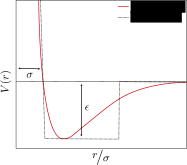
\includegraphics[width=\columnwidth]{figs/well-potential.pdf}
    \caption{The square-well and the Lennard-Jones potentials are graphically shown vs. the radial distance from the particle.
    }
    \label{fig:well-potential}
  \end{figure}

\subsection{Square-Well Fluid}
The square-well fluid is a system of particles whose interactions are governed by a square-well
potential~\cite{singh2003surface, barker2004perturbationSW} as shown in Fig.~\ref{fig:well-potential}.  The square-well potential is an ideal test-bed
for Monte Carlo methods as it is a simple model for a liquid, which includes both attractive and repulsive
interactions~\cite{barker1967-SW-perturbation, vega1992phase}. The potential $U(\textbf{r})$ for such a system
is given by
\begin{equation}
 U(\textbf{r})=\begin{cases} \infty &
 \lvert\textbf{r}\rvert< \sigma\\-\epsilon &
 \sigma<\lvert\textbf{r}\rvert<\lambda\sigma\\0 &
 \lvert\textbf{r}\rvert > \lambda\sigma\end{cases}
\end{equation}
where $\sigma$ is the hard-sphere diameter of the particle, $\lambda$ is the reduced range of the potential well, and $\epsilon$ is its depth.

\subsection{2D Ising Model}
The 2D Ising spin-lattice system is widely used as a test-bed when benchmarking or comparing Monte-Carlo
methods~\cite{ferdinand1969bounded, wang1999transition, trebst2004optimizing}. The \nth{2} order phase
transition behavior and the ability to directly calculate the exact solution for finite
lattices~\cite{beale1996exact} make the system sufficiently interesting for such theoretical comparisons.
The Hamiltonian for the periodic 2D square lattice ferromagnetic Ising model with nearest
neighbor interactions~\cite{landau2004new} cab be written as the following:
\begin{align}
\mathcal{H} = -\sum_{\braket{i,j}} \sigma_i \sigma_j - h \sum_i \sigma_i
\end{align}
The $N\times N$ spin system can take on values of $\sigma_i = \pm 1$
for up or down spins respectively. In the absence of a magnetic field ($h =
0$), we can write the Hamiltonian as follows~\cite{onsager1944crystal,
kaufman1949crystal}:
\begin{align}
\mathcal{H} = -\sum_{\braket{i,j}} \sigma_i \sigma_j
\end{align}
where the sum is over nearest neighbor spin sites.

\subsection{Lennard-Jones Clusters}
Lennard-Jones cluster systems are widely used as a challenging test-bed when comparing Monte-Carlo
methods~\cite{doye1998thermodynamics, poulain2006performances, martiniani2014superposition}. The potential
energy for interacting atomic particles can be written as follows and can visually be seen in Fig.~\cite{fig:well-potential}:
\begin{align}
U = 4\epsilon \left[\left( \sigma/r \right)^{12} - \left( \sigma/r \right)^{6}\right]
\end{align}
A number of challenges exist when trying to accurately simulate the density of states of a cluster system.
Narrow potential energy funnels~\cite{mandelshtam2006multiple, wales1997global} and low temperature solid-solid
transitions~\cite{neirotti2000phase, calvo2000phase, calvo2000entropic} make predicting thermodynamic properties
such as heat capacity an extremely difficult process. In addition, since flat-histogram methods explore all
energies and all temperatures it is possible that for high temperatures a large cluster volume is possible
(which could lead to boil-off of the particles). A `constraining' sphere with radius $R_c$ is used to prevent
this but it is usually empirically determined, further complicating the simulation process.

\section{Gas Storage and Delivery in Metal-Organic Frameworks}


Due to their low volumetric energy density at ambient conditions, both hydrogen
and natural gas are challenging to economically store onboard environmentally
sustainable vehicles~\cite{mason2014evaluating, sircar2002pressure}. One
strategy to densify these gases is to pack the fuel tank with a porous
material~\cite{schoedel2016role}. Metal-organic frameworks (MOFs) are tunable, nanoporous
materials with large internal surface areas and show considerable promise for
densifying gases~\cite{makal2012methane,mason2014evaluating,
suh2011hydrogen,garcia2018benchmark, schoedel2016role}. The US Department of
Energy (DOE) has set volumetric deliverable capacity targets~\cite{simon2015materials, h2targetsDOE} which, if met, would help to enable 
commercial adoption of hydrogen/natural gas as
transportation fuels. Many have attempted to establish theoretical upper bounds
on the deliverable capacity via pressure-swing adsorption using simplified
models of the gas-substrate and gas-gas interaction~\cite{gomez2014exploring, 
gomez2017impact, kaija2018high, lee2019predicting}; none have
established a rigorous upper bound on the deliverable capacity.

We present a theoretical upper bound on the deliverable capacity of a
rigid material via an isothermal pressure-swing. To provide an extremum, we
consider a substrate that provides a spatially uniform potential energy field
for the gas. Our bound is unique in that it directly relies on experimentally
measured properties of the (real) bulk gas, without making approximations.
We conclude that the goals set by the US DOE for natural gas and hydrogen
storage are theoretically possible, but sufficiently close to the upper bound
as to be impractical for any real porous material. However, limitations to the
scope of applicability of our upper bound guide future material development 
efforts. Firstly, one could heat the adsorbent to drive off residual gas when
the pressure diminishes~\cite{gomez2014exploring}. Secondly, the fundamental
physics of our upper bound do not pertain to any material that changes its
structure in response to adsorbed gas, suggesting that flexible materials could
still satisfy the DOE targets~\cite{schneemann2014flexible, choi2008broadly, mason2015methane}.

% Now add why a multidimensional 2D SAD would help and how we are working toward it.
Due to the difficulty in designing the ``ideal'' MOF for gas storage
applications, computational methods are necessary that can predict the
associated thermodynamic properties of interest. While SAD is an invaluable tool
for calculating a single isotherm (at a given density), an even more powerful
method is necessary for determining the best MOF for gas storage applications.
A multidimensional SAD would allow researchers to compute all properties of
interest for all densities and temperatures. Our research has
yielded a robust method that has been tested on multiple systems and can be
extended into a higher dimension formulation. 

\section{Summary}
We have provided the background necessary for understanding the various
flat-histogram methods and the various applied test systems. In the following
chapters, we detail our manuscripts and the method SAD applied to the various
physical test systems. We test SAD against a variety of other weight-based
flat-histogram methods on the square-well fluid, a Lennard-Jones cluster, and
the 2D Ising model. Each of these systems provides unique challenges to our
newly developed method SAD and convergence robustness is determined best by the
application to multiple systems.

We are currently working on two extensions which will enable a multidimensional
SAD. The first is (i) adaptive interpolation histogram binning. This technique
will decrease the simulation time by orders of magnitude. The second is (ii) a
version of SAD that simulates ``number'' space rather than energy space. These
two extensions will enable all densities to be extracted and should decrease
simulation time. The development of 2D SAD will provide a powerful way for
researchers to work toward enabling environmentally sustainable light vehicle
storage.